\documentclass[10pt,letter]{article}
\usepackage{amsmath}
\usepackage{amssymb}
\usepackage[makeroom]{cancel}
\usepackage{graphicx}
\usepackage{setspace}
\usepackage{stmaryrd}
\usepackage{xcolor}
\def\fatbar{\talloblong}
\onehalfspacing
\usepackage{fullpage}
\newcommand{\R}{\mathbb{R}}	
\newcommand{\inner}{\langle\cdot,\cdot\rangle}
\newcommand{\inr}[2]{\langle #1, #2\rangle}
\newcommand\norm[1]{\left\lVert#1\right\rVert}

\graphicspath{ {images/} }

\begin{document}


\title{CS142 Homework Set \#7 Solutions}

\author{Timur Kuzhagaliyev}

%\date{21st November, 2017}
 
\maketitle 

\section*{Problem 1}

To verify that the algorithm would still be correct, we need to show that all of the previous safety properties still hold:

\begin{enumerate}
\item Learners learn at most one value.
\item Learners learn only proposed values.
\item All learners learn the same unchanging value (given a particular learner learns anything at all).
\end{enumerate}

Clearly, property \#2 is still satisfied since we're not changing the nature of the proposed values themselves, nor how values are accepted. We only need to focus on properties \#1 and \#3.

Note that in Paxos algorithm, acceptor only sends out a \textbf{granted(...)} message if the new $n$ received through \textbf{prepare(n)} is strictly higher than the current $highest\_prepare\_n$. Since in our case at most two proposals can have the same $n$, this scenario simplifies down to a race condition between two proposers with different values but same number $n$ - whoever manages to get its \textbf{prepare(n)} message to the acceptor first will end up getting the \textbf{granted(...)} message back.

To clarify the above - the proposer, say $A$, will send out its \textbf{accept(...)} message $iff$ it receives a \textbf{granted(...)} message that satisfies certain properties. If \textbf{prepare(n)} of another proposer $B$ will reach the acceptor faster than that of $A$, the acceptor would already have $n$ stored and hence will reject $A$'s \textbf{prepare(n)}. In this case $A$ will stop exchanging messages with the acceptor in question and hence cannot cause it to fail. 

Can this race condition violate safety properties \#1 and \#3? It cannot, because after this initial race condition has settled (in favour of one proposal or another, for each relevant acceptor), every agent in the system will continue normal execution of the algorithm, which we know does satisfy the safety properties. Therefore the algorithm would still be correct.

\pagebreak

\section*{Problem 2}

It must be noted that Paxos algorithm does not guarantee progress. That said, the algorithm would still satisfy the safety conditions if any number of acceptors fail. Intuitively, this is true because Paxos algorithm was designed to solve this exact problem.

This can also be shown by following the original proof of algorithm's correctness. The original proof (for the case when all acceptors are working) hinges on the fact that any two majority sets would have at least one common acceptor. As guaranteed by the algorithm, this common acceptor can accept different proposals, but all these proposals will necessary have the same value. Therefore this common acceptor guarantees that any majority acceptor set the learner can learn from would have the same value.

If we decrease the total number of acceptors but use the same number as the lower bound for the majority set, we simply make the algorithm "stricter". Each majority set will now have a greater overlap (more common acceptors), and these common acceptors will carry out their usual role of ensuring all majority sets are in sync.

This can obviously have detrimental effects on progress (especially if number of remaining agents is smaller than our bound on majority set), but it does not violate the safety property -  if anything, the algorithm becomes more "safe". Therefore the algorithm would still be correct.

\section*{Problem 3}

As a reminder, safety properties of the Paxos algorithm:

\begin{enumerate}
\item Learners learn at most one value.
\item Learners learn only proposed values.
\item All learners learn the same unchanging value (given a particular learner learns anything at all).
\end{enumerate}

The algorithm proposed in the question would not work. $Acceptor's\; choice$ plays a very important role of ensuring that if the acceptor has accepted some proposal $p$, any subsequent proposal $p^*$ accepted by the same agent will have the same value as $p$. Safety properties \#1 and \#3 rely on this fact very heavily: in the original Paxos algorithm, if a learner has learnt some value from a majority set of acceptors, it knows that these acceptors will never change the value they've learnt (although they can accept new proposals), and hence the learner will never learn another value.

In the modified algorithm, this assumption would be invalid. Here is a simple counter example: Consider the case with 2 proposers, $P_A$ and $P_B$, 3 acceptors, and some arbitrary non-zero number of learners. First, $P_A$ sends out a prepare message to all acceptors. Since this is the first perpare mesasge they get, all acceptors accept it and reply with \textbf{granted(...)}. $P_A$ then goes on to send out its proposal $p_a$, this proposal gets accepted by all acceptors and learners learn the value of $p_a$.

Now, $P_B$ sends out its own prepare messages with $n$ higher than the one $P_A$ used it. Following the normal Paxos algorithm, it gets to propose its own value. Since $P_B$ is no longer bound by $Acceptor's\; choice$ choice, $P_B$ proposes some $p_b \neq p_a$. Next, $p_b$ gets accepted by all acceptors and subsequently learnt by all learners. This implies that every learner has learnt 2 distinct values, which violates safety properties \#1 and \#3.

\section*{Problem 4}

\paragraph{a)} Let's denote $A$'s transaction as $t_A$ and $B$'s transaction as $t_B$. Assuming $A$ and $B$ cast transactions at the same time, the will effectively split the network into 2 parts: one part would accept $t_A$ and the other would accept $t_B$, while rejecting the other. This separation is show in Figure \ref{fig:split}.

\begin{figure}[h!]
\centering
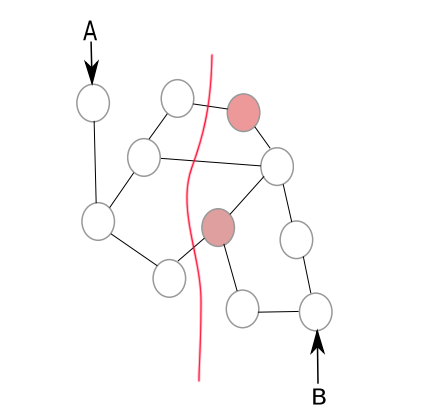
\includegraphics[scale=0.5,keepaspectratio]{hw8_problem4_a}
\caption{Network split into nodes that accepted $t_A$ (left) or $t_B$ (right)}
\label{fig:split}
\end{figure}

Now, for either $A$ or $B$ to get accepted, the other transaction needs to get orphaned (i.e. no node in the network should be considering it). In the case of $t_A$, this can happen if at least one node that accepted $t_A$ mines a block and no nodes that have accepted $t_B$ mine a block. Similar scenario holds for $t_B$.

We know that each node has the same computational power, so the probability of mining a block first simplifies to the proportion of nodes each side contains. Therefore:
\begin{align*}
\textrm{Pr($t_A$ gets accepted)}\; &= \frac{5}{11}
\\
\textrm{Pr($t_B$ gets accepted)}\; &= \frac{6}{11}
\end{align*}

\paragraph{b)} Adjust the proportions based on red nodes with twice the computational power:
\begin{align*}
\textrm{Pr($t_A$ gets accepted)}\; &= \frac{5}{13}
\\
\textrm{Pr($t_B$ gets accepted)}\; &= \frac{8}{13}
\end{align*}

\pagebreak

\section*{Problem 5}

\paragraph{a)} The final probability of B getting orphaned can be seen below. I've colour coded the equation to make the logic easier to follow.

\begin{figure}[h!]
\centering
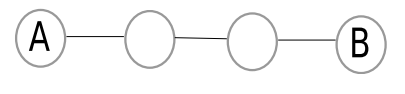
\includegraphics[scale=0.5,keepaspectratio]{hw8_problem5_a}
\caption{Network for Problem 5 (a).}
\end{figure}
\begin{align*}
P = \textcolor{red}{p(1-p)^2 * (1 - p(1-p))} + \textcolor{blue}{p^2(1-p) * \frac{1}{2} * p(1-p)}
\end{align*}

Let's denote the nodes as $A, C, D, B$ respectively. Since in first round $A$ and $B$ each mined a block, $A, C$ start out with chain $A1$ and $D, B$ start out with chain $B1$. There are 8 possible outcomes in round 2, since we only need to consider nodes $C, D, B$. There are only 2 scenarios for round 2 after which B can get orphaned in round 3.

One scenario is when only $C$ mines a block in round 2, with probability $p(1-p)^2$. This means that in round 3, $C, D$ will both have chain $A1\rightarrow C2$, while $B$ will still have $B1$. Now, in round 3, the only scenario where $B$ \textbf{does not} get orphaned is when $B$ mines a block and $D$ does not, with probability of $p(1-p)$. The complement is $1 - p(1-p)$. Now, if we multiply together the probability of original round 2 scenario and this complement, we get the red part of the equation.

Second scenario in round 2 that can make B get orphaned in round 3 is when $C, B$ but not $D$ mine a block, with probability $p^2(1-p)$. Now, it's unclear whose chain $D$ will accept - I will assume that there's a 50/50 chance of each chain getting accepted. If $B$'s chain is accepted, we're good, but if $C$'s chain is accepted $B$ can still be orphaned in round 3. In this case, $D$ will have $A1->C2$ and $B$ will have $B1->B2$. B gets orphaned when $D$ mines a block in round 3 and $B$ does not, which can happen with probability $p(1-p)$. Multiplying the probability of original scenario in round 2, the chance of $C$'s chain getting accepted over $B$'s, and, finally, the probability of $B$ getting orphaned we get the blue part of the equation.

\paragraph{b)} In part (a) of the question, we needed $C$ to mine a block in round 2 to have a non-zero chance of $B$ being orphaned in round 3. Now, since there are more nodes directly connected to $A$, which are also connected to $D$, the chance of the new block being mined in round 2 and $B$ getting orphaned in round 3 has increased. This follows from both the increased computational power and combined probability of the 2 new nodes.

\begin{figure}[h!]
\centering
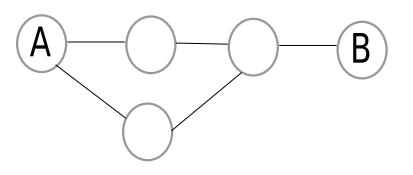
\includegraphics[scale=0.5,keepaspectratio]{hw8_problem5_b}
\caption{Network for Problem 5 (b).}
\end{figure}

As a result, $B$ is more likely to get orphaned because it is connected to a smaller number of nodes than someone else on the network who also mines a block at the same time. From this notion we can conclude that the smaller the degree of some particular node is, the more likely are its blocks to get orphaned.

\end{document}